\documentclass[semifinal]{cpecmu}

%% This is a sample document demonstrating how to use the CPECMU
%% project template. If you are having trouble, see "cpecmu.pdf" for
%% documentation.

\projectNo{P040-2}
\acadyear{2023}

\titleTH{สงคราม Doggy Kitty}
\titleEN{Doggy Kitty War}

\author{นายกฤษณพงศ์ เทพวีระกุล}{Kritsanaphong Tepwerakul}{630610714}
\author{นางสาววรนุช กิจการ}{Woranut Kitchakan}{630610760}

\cpeadvisor{navadon}
\cpecommittee{karn}
\cpecommittee{sakgasit}

%% Some possible packages to include:
\usepackage[final]{graphicx} % for including graphics

%% Add bookmarks and hyperlinks in the document.
\PassOptionsToPackage{hyphens}{url}
\usepackage[colorlinks=true,allcolors=Blue4,citecolor=red,linktoc=all]{hyperref}
\def\UrlLeft#1\UrlRight{$#1$}

%% Needed just by this example, but maybe not by most reports
\usepackage{afterpage} % for outputting
\usepackage{pdflscape} % for landscape figures and tables. 

%% Some other useful packages. Look these up to find out how to use
%% them.
% \usepackage{natbib}    % for author-year citation styles
% \usepackage{txfonts}
% \usepackage{appendix}  % for appendices on a per-chapter basis
% \usepackage{xtab}      % for tables that go over multiple pages
% \usepackage{subfigure} % for subfigures within a figure
% \usepackage{pstricks,pdftricks} % for access to special PostScript and PDF commands
% \usepackage{nomencl}   % if you have a list of abbreviations
\usepackage{multirow}
\usepackage{tabularx}
\usepackage{array}
\usepackage{cite}
%% if you're having problems with overfull boxes, you may need to increase
%% the tolerance to 9999
% \tolerance=9999
\bibliographystyle{plain}
% \bibliographystyle{IEEEbib}

% \renewcommand{\topfraction}{0.85}
% \renewcommand{\textfraction}{0.1}
% \renewcommand{\floatpagefraction}{0.75}

%% Example for glossary entry
%% Need to use glossary option
%% See glossaries package for complete documentation.
\ifglossary
  \newglossaryentry{lorem ipsum}{
    name=lorem ipsum,
    description={derived from Latin dolorem ipsum, translated as ``pain itself''}
  }
\fi

%% Uncomment this command to preview only specified LaTeX file(s)
%% imported with \include command below.
%% Any other file imported via \include but not specified here will not
%% be previewed.
%% Useful if your report is large, as you might not want to build
%% the entire file when editing a certain part of your report.
% \includeonly{chapters/intro,chapters/background}

\begin{document}
\maketitle
\makesignature

\ifproject
\begin{abstractTH} % บทคัดย่อ (ไทย)

\quad โครงการพัฒนาเกม Doggy Kitty War เป็นเกมแนววางแผนกลยุทธ์แบบ Real time (Real Time Strategy : RTS) โดยจะเป็นเกมเล่น 2 คน (Two-player game) ผู้เล่นจะต้องวางแผนกลยุทธ์การจัดการทรัพยากรภายในเกม และเอาชนะฝั่งตรงข้ามโดยการทำลายฐานทัพของอีกฝ่าย

\end{abstractTH}

\begin{abstract} % บทคัดย่อ (อังกฤษ)

\quad Doggy Kitty War is a Real Time Strategy game (RTS). This game will be a two-playergame. Players will have to plan strategies for managing for resources within
the game and conquer the enemy by destroying their bases.

\end{abstract}

\iffalse
\begin{dedication}
This document is dedicated to all Chiang Mai University students.

Dedication page is optional.
\end{dedication}
\fi % \iffalse

\begin{acknowledgments}

\qquad โครงการพัฒนาเกม Doggy Kitty War จะไม่สามารถประสบความสําเร็จได้โดยไม่ได้รับความกรุณาจากผู้ที่มีประสบการณ์และความรู้ในการดูแลและสนับสนุนโครงการ เราขอขอบคุณอาจารย์ที่ปรึกษาโครงการ
ผศ.ดร.นวดนย์ คุณเลิศกิจ ที่ให้คําแนะนํา ความรู้และความช่วยเหลือแก่ผู้พัฒนา รวมถึงการสนับสนุนทรัพยากรต่างๆ ที่จําเป็นต่อการดําเนินโครงการของเรา

\enskip เราขอขอบคุณภาควิชาวิศวกรรมคอมพิวเตอร์คณะวิศวกรรมศาสตร์มหาวิทยาลัยเชียงใหม่ ที่เอื้อเฟื้อ\\สถานที่และทรัพยากรที่จําเป็นในการทํางาน เราหวังว่าจะได้เป็นส่วนหนึ่งในการสร้างพัฒนาและนําเสนอเทคโนโลยี
ใหม่ๆในอนาคต

\acksign{2024}{3}{01}
\end{acknowledgments}%
\fi % \ifproject

\contentspage

\ifproject
\figurelistpage

\tablelistpage
\fi % \ifproject

% \abbrlist % this page is optional

% \symlist % this page is optional

% \preface % this section is optional


\pagestyle{empty}\cleardoublepage
\normalspacing \setcounter{page}{1} \pagenumbering{arabic} \pagestyle{cpecmu}

\chapter{\ifenglish Introduction\else บทนำ\fi}

\section{\ifenglish Project rationale\else ที่มาของโครงงาน\fi}

\qquad ในปัจจุบันนี้เกมเป็นสื่อที่เข้าถึงง่ายและได้รับความนิยมสูงไม่ว่าจะในเด็กหรือผู้ใหญ่ อีกทั้งเกมยังมีการจัดการแข่งขันเป็นกีฬาและมีเงินรางวัล ทําให้เกมที่นอกจากจะเป็นสื่อบันเทิงแล้ว 
ยังเป็นอีกแหล่งทําเงินและกระตุ้นเศรษฐกิจด้วย ในด้านของความบันเทิง เกมทําให้ผู้เล่นได้แสดงทักษะต่างๆที่เป็น soft
skill อย่างเช่นการวางแผน การมีปฏิสัมพันธ์กับผู้อื่น การทํางานเป็นทีม ความสามัคคี และการแก้ไขปัญหาเฉพาะหน้า

\enskip จากการศึกษา soft skill ที่สามารถนําไปใช้ในสถาณการณ์ต่างๆได้ หนึ่งใน soft skill ที่สําคัญต่อการทํางานคือ การวางแผนและการบริหารจัดการทรัพยากร ผู้จัดทําจึงมีความสนใจในการจัดทําเกมที่ทําให้ผู้เล่น
นั้นสามารถแสดง soft skill ในเรื่องการวางแผน ดังนั้นผู้จัดทําจึงได้มีแนวคิดที่จะทําเกมแนว RTS (Real Time Strategy) เพื่อให้ผู้เล่นได้ฝึกทักษะการวางแผน การจัดการทรัพยากรที่มีอย่างจํากัดรวมถึงบังคับ unit 
ให้ไปต่อสู้หรือแก้ปัญหาที่อาจเกิดจากฝ่ายตรงข้าม
\section{\ifenglish Objectives\else วัตถุประสงค์ของโครงงาน\fi}
\begin{enumerate}
    \item เพื่อออกแบบเกมให้ผู้เล่นได้เกิดความสนุกสนาน เพลิดเพลิน
    \item เพื่อให้ผู้เล่นได้ฝึกฝนการคิดและวางแผนในการบริหารจัดการทรัพยากร
\end{enumerate}

\section{\ifenglish Project scope\else ขอบเขตของโครงงาน\fi}

\subsection{\ifenglish Hardware scope\else ขอบเขตด้านฮาร์ดแวร์\fi}
\begin{enumerate}
    \item พัฒนาเกมที่สามารถเล่นบนคอมพิวเตอร์ส่วนตัว หรือคอมพิวเตอร์พกพา
    \item ใช้แป้นพิมพ์และเมาส์ในการควบคุมภายในเกม
\end{enumerate}
\subsection{\ifenglish Software scope\else ขอบเขตด้านซอฟต์แวร์\fi}
พัฒนาเกม 3 มิติ โดยจะเป็นการเล่นที่รองรับผู้เล่น 2 คน (Two-player game)

\section{\ifenglish Expected outcomes\else ประโยชน์ที่ได้รับ\fi}
\begin{enumerate}
    \item ผู้เล่นจะได้รับประสบการณ์และความรู้ในด้านการวางแผนและการจัดการทรัพยากร
    \item ผู้เล่นจะได้รับความบันเทิง ความสนุกสนานและความเพลิดเพลิน
\end{enumerate}

\section{\ifenglish Technology and tools\else เทคโนโลยีและเครื่องมือที่ใช้\fi}

\subsection{\ifenglish Hardware technology\else เทคโนโลยีด้านฮาร์ดแวร์\fi}
\begin{enumerate}
    \item คอมพิวเตอร์พกพา ใช้ในการพัฒนาเกม
\end{enumerate}
\subsection{\ifenglish Software technology\else เทคโนโลยีด้านซอฟต์แวร์\fi}
\begin{enumerate}
    \item Unity สําหรับการพัฒนาเกม
    \item Unity asset
    \item Microsoft Visual Studio Community 2022
    \item ภาษา C\# 
\end{enumerate}

\section{\ifenglish Project plan\else แผนการดำเนินงาน\fi}

\begin{plan}{6}{2023}{3}{2024}
    \planitem{6}{2023}{6}{2023}{ศึกษาค้นคว้ากําหนดหัวข้อ}
    \planitem{7}{2023}{12}{2023}{ออกแบบเนื้อเรื่องและระบบภายในเกม}
    \planitem{6}{2023}{3}{2024}{ศึกษาการใช้Unity}
    \planitem{10}{2023}{3}{2024}{พัฒนาโปรแกรม}
    \planitem{12}{2023}{3}{2024}{ทดสอบและแก้ไขข้อบกพร่อง}
    \planitem{3}{2024}{3}{2024}{จัดทํารายงานสรุปผล}
\end{plan}

\section{\ifenglish Roles and responsibilities\else บทบาทและความรับผิดชอบ\fi}
\begin{itemize}
    \item นายกฤษณพงศ์ เทพวีระกุล : Game Developer 
    \item นางสาววรนุช กิจการ : Project Manager, Game Designer, Tester
\end{itemize}
\section{\ifenglish%
Impacts of this project on society, health, safety, legal, and cultural issues
\else%
ผลกระทบด้านสังคม สุขภาพ ความปลอดภัย กฎหมาย และวัฒนธรรม\fi}

\qquad Doggy Kitty War เป็นเกม Real Time Strategy ที่จะเป็นตัวช่วยเสริมสร้าง ฝึกฝนทักษะการวางแผนและการจัดการทรัพยากร
 ซึ่งนําไปประยุกต์เข้ากับการทํางานได้ ภายในเกมมีฉากต่อสู้, ฉากการตายของ Unit/Hero แต่ด้วยเนื้อหาในเกมที่มีภาพแบบไม่สมจริง 
 ดังนั้นจึงไม่มีผลกระทบต่อผู้เล่นที่มีความอ่อนไหวต่อเนื้อหาที่รุนแรงภายในเกม
\chapter{\ifenglish Background Knowledge and Theory\else ทฤษฎีที่เกี่ยวข้อง\fi}

\quad การจัดทําโครงงานพัฒนาเกมนี้ ซึ่งเป็นเกม RTS ที่ควบคุมการเล่นผ่านทางแป้นพิมพ์ และเมาส์ เบื้องต้นในการพัฒนาโปรแกรมนั้นได้ศึกษาค้นคว้าเกี่ยวกับ Game engine ที่ใช้ในการพัฒนาเกม 
และศึกษาเกี่ยวกับประเภทของเกม เนื้อหาในบทนี้จะอธิบายส่วนต่างๆที่เกี่ยวข้องกับโครงงาน เพื่อเพิ่มความเข้าใจในบทถัดไปได้ง่ายมากยิ่งขึ้น

\section{Unity (game engine)}

\qquad Unity คือซอฟต์แวร์สําหรับใช้เพื่อสําหรับการพัฒนาซอฟต์แวร์และการจําลองต่างๆ เป็นโปรแกรมที่มีความสามารถหลากหลาย ได้แก่ การสร้างเกม 2 มิติ, 3 มิติ การสร้าง AR, VR 
สามารถส่งแอพพลิเคชั่นได้ทั้งระบบ Windows, iOS และ Android

\enskip ในการเขียนโปรแกรมเกมนั้น Unity สามารถเขียนด้วยภาษา C++ ได้ แต่ยังไงก็ตามผู้พัฒนาสามารถเขียนภาษา C++ ได้แค่ในส่วนการทํางานพื้นหลังเท่านั้น เช่น ระบบเสียง, บริการพื้นหลัง, ปลั๊กอิน ซึ่งการ
ปฏิสัมพันธ์กับ Engine ทําได้ค่อนข้างน้อย ดังนั้นภาษา C\# จึงเหมาะสมสําหรับกับการใช้ในการพัฒนามากกว่า


\section{เกมกลยุทธ์}
\subsection{เกมกลยุทธ์แบบเรียลไทม์ (Real-Time Strategy : RTS)}

\qquad เป็นประเภทย่อยของวิดีโอเกมกลยุทธ์ (Strategy game) เกมกลยุทธ์แบบเรียลไทม์ช่วยให้ผู้เล่นทุกคนสามารถเล่นเกมแบบ “Real-time” ได้พร้อมกัน

\enskip เป็นเกมที่มุ่งเน้นไปที่การใช้ทรัพยากรเพื่อสร้าง unit และเอาชนะคู่ต่อสู้ เกมกลยุทธ์แบบเรียลไทม์มักจะถูกเปรียบเทียบกับเกมวางแผนแบบ turn based ซึ่งผู้เล่นแต่ละคนมีเวลาพิจารณาอย่างรอบคอบในการเคลื่อนที่ครั้งต่อไปโดยไม่ต้องกังวลเกี่ยวกับการกระทําของฝ่ายตรงข้าม 
แต่ในเกมกลยุทธ์แบบเรียลไทม์ผู้เล่นจะต้องพยายามปกป้องฐานและเริ่มการโจมตีในขณะที่รู้ว่าฝ่ายตรงข้ามกําลังต่อสู้เพื่อทําสิ่งเดียวกัน

\subsection{การเล่นเกม}

\qquad ในเกมกลยุทธ์แบบเรียลไทม์ทั่วไปหน้าจอจะแบ่งออกเป็นพื้นที่แผนที่ที่แสดงโลกของเกม, ภูมิประเทศและสิ่งปลูกสร้าง ผู้เล่นมักจะได้เล่นในมุมมองจากที่สูง 
ควบคุมโดยการเลื่อนหน้าจอและออกคําสั่งด้วยเมาส์และอาจใช้แป้นพิมพ์ลัด (short key)

\enskip การเล่นเกมโดยทั่วไปประกอบด้วยผู้เล่นที่อยู่ในตําแหน่งใดที่หนึ่งในแผนที่โดยมี unit ไม่กี่ unit หรือ building ที่สามารถสร้าง unit / building อื่นได้ 
โดยมักจะให้ผู้เล่นสร้างสิ่งก่อสร้างที่เฉพาะเจาะจงเพื่อปลดล็อค unit ในขั้นที่สูงขึ้น เกม RTS ต้องการให้ผู้เล่นสร้างกองทัพ 
(ตั้งแต่ unit เล็ก ๆ ไม่เกิน 2 unit ไปจนถึง unit หลายร้อย unit) ใช้เพื่อป้องกันตัวเองจากการโจมตีของศัตรูหรือกําจัดศัตรูที่ครอบครองฐานที่มีกําลังการผลิต unit เป็นของตัวเอง 
ในบางครั้งเกม RTS จะมีจํานวน unit ที่กําหนดไว้ล่วงหน้าเพื่อให้ผู้เล่นควบคุมและไม่อนุญาตให้สร้าง unit เพิ่มเติมเกินจากที่กําหนดไว้

% \section{Third section}
% Section 3 text. The dielectric constant\index{dielectric constant}
% at the air-metal interface determines
% the resonance shift\index{resonance shift} as absorption or capture occurs
% is shown in Equation~\eqref{eq:dielectric}:

% \begin{equation}\label{eq:dielectric}
% k_1=\frac{\omega}{c({1/\varepsilon_m + 1/\varepsilon_i})^{1/2}}=k_2=\frac{\omega
% \sin(\theta)\varepsilon_\mathit{air}^{1/2}}{c}
% \end{equation}

% \noindent
% where $\omega$ is the frequency of the plasmon, $c$ is the speed of
% light, $\varepsilon_m$ is the dielectric constant of the metal,
% $\varepsilon_i$ is the dielectric constant of neighboring insulator,
% and $\varepsilon_\mathit{air}$ is the dielectric constant of air.

% \section{About using figures in your report}

% define a command that produces some filler text, the lorem ipsum.
% \newcommand{\loremipsum}{
%   \textit{Lorem ipsum dolor sit amet, consectetur adipisicing elit, sed do
%   eiusmod tempor incididunt ut labore et dolore magna aliqua. Ut enim ad
%   minim veniam, quis nostrud exercitation ullamco laboris nisi ut
%   aliquip ex ea commodo consequat. Duis aute irure dolor in
%   reprehenderit in voluptate velit esse cillum dolore eu fugiat nulla
%   pariatur. Excepteur sint occaecat cupidatat non proident, sunt in
%   culpa qui officia deserunt mollit anim id est laborum.}\par}

% \begin{figure}
%   \centering

%   \fbox{
%      \parbox{.6\textwidth}{\loremipsum}
%   }

%   % To include an image in the figure, say myimage.pdf, you could use
%   % the following code. Look up the documentation for the package
%   % graphicx for more information.
%   % \includegraphics[width=\textwidth]{myimage}

%   \caption[Sample figure]{This figure is a sample containing \gls{lorem ipsum},
%   showing you how you can include figures and glossary in your report.
%   You can specify a shorter caption that will appear in the List of Figures.}
%   \label{fig:sample-figure}
% \end{figure}

% Using \verb.\label. and \verb.\ref. commands allows us to refer to
% figures easily. If we can refer to Figures
% \ref{fig:walrus} and \ref{fig:sample-figure} by name in the {\LaTeX}
% source code, then we will not need to update the code that refers to it
% even if the placement or ordering of the figures changes.

% \loremipsum\loremipsum

% This code demonstrates how to get a landscape table or figure. It
% uses the package lscape to turn everything but the page number into
% landscape orientation. Everything should be included within an
% \afterpage{ .... } to avoid causing a page break too early.
% \afterpage{
%   \begin{landscape}
%   \begin{table}
%     \caption{Sample landscape table}
%     \label{tab:sample-table}

%     \centering

%     \begin{tabular}{c||c|c}
%         Year & A & B \\
%         \hline\hline
%         1989 & 12 & 23 \\
%         1990 & 4 & 9 \\
%         1991 & 3 & 6 \\
%     \end{tabular}
%   \end{table}
%   \end{landscape}
% }

% \loremipsum\loremipsum\loremipsum

% \section{Overfull hbox}

% When the \verb.semifinal. option is passed to the \verb.cpecmu. document class,
% any line that is longer than the line width, i.e., an overfull hbox, will be
% highlighted with a black solid rule:
% \begin{center}
% \begin{minipage}{2em}
% juxtaposition
% \end{minipage}
% \end{center}

\section{\ifenglish%
\ifcpe CPE \else ISNE \fi knowledge used, applied, or integrated in this project
\else%
ความรู้ตามหลักสูตรซึ่งถูกนำมาใช้หรือบูรณาการในโครงงาน\fi}

\qquad ในการจัดทำโครงงานนี้ มีหลายหัวข้อที่ผู้พัฒนานั้นยังไม่มีความชำนาญ และยังขาดประสบการณ์ 
จึงได้นำความรู้ที่ได้รับจากการเรียนการสอนตามหลักสูตรของวิศวกรรมคอมพิวเตอร์ มหาวิทยาลัยเชียงใหม่มาใช้ ดังนี้
\begin{enumerate}
  \item Object-Oriented Programming (OOP)
  
  \qquad ใช้ช่วยในการพัฒนาโปรแกรม,การเขียนโปรแกรมเชิงวัตถุ ทำให้ object ต่างๆภายในเกมสามารถทำงานได้อย่างถูกต้องและมีประสิทธิภาพ
  \item Algorithms
  
  \qquad ช่วยกำหนดทิศทางและเป้าหมายในพัฒนาโปรแกรม วางแผนแก้ไขปัญหาอย่างเป็นขั้นตอน
  \item Software Engineering
  
  \qquad ช่วยทำให้การพัฒนาซอฟต์แวร์เกิดขึ้นอย่างเป็นระบบ
  \item Human-computer interaction (HCI) 
  
  \qquad ช่วยในการออกแบบโปรแกรม เพื่อสนับสนุนประสบการณ์การใช้งานของผู้ใช้ (user eperience)
\end{enumerate}

\section{\ifenglish%
Extracurricular knowledge used, applied, or integrated in this project
\else%
ความรู้นอกหลักสูตรซึ่งถูกนำมาใช้หรือบูรณาการในโครงงาน\fi}

\qquad ในการจัดทำโครงงานนี้ นอกเหนือจากความรู้ตามหลักสูตรของทางมหาวิทยาลัย ผู้พัฒนายังได้ไปศึกษาเนื้อหานอกหลักสูตรเพื่อนำมาใช้ในการพัฒนาโปรแกรม ดังนี้

\begin{enumerate}
  \item MDA framework 
  
  \qquad ช่วยในการออกแบบเกม เพื่อให้ผู้เล่นเกิดความสนุกไปกับเกม
  \item การพัฒนาเกมด้วย Unity engine
  
  \qquad เพื่อช่วยอำนวยความสะดวกให้กับการพัฒนาเกม
\end{enumerate}

\chapter{\ifproject%
\ifenglish Project Structure and Methodology\else โครงสร้างและขั้นตอนการทำงาน\fi
\else%
\ifenglish Project Structure\else โครงสร้างของโครงงาน\fi
\fi}

\qquad ในบทนี้จะกล่าวถึงเนื้อเรื่องของเกม, เกมเพลย์, วิธีการเล่นเกม เพื่อให้ผู้เล่นได้เข้าใจเป้าหมายและวิธีการเล่นของเกมนี้มากยิ่งขึ้น

% \makeatletter

% % \renewcommand\section{\@startsection {section}{1}{\z@}%
% %                                    {13.5ex \@plus -1ex \@minus -.2ex}%
% %                                    {2.3ex \@plus.2ex}%
% %                                    {\normalfont\large\bfseries}}

% \makeatother
% %\vspace{2ex}
% % \titleformat{\section}{\normalfont\bfseries}{\thesection}{1em}{}
% % \titlespacing*{\section}{0pt}{10ex}{0pt}

\section{เนื้อเรื่อง}

\qquad เกมมีเนื้อเรื่องเกี่ยวกับ ในป่าแห่งหนึ่งที่มีสองเผ่าที่อาศัยอยู่ร่วมกัน คือเผ่า Doggy และเผ่า Kitty ในอดีตทั้งสองเผ่าอยู่ร่วมกันอย่างสันติ โดยที่แบ่งปันทรัพยากรซึ่งกันและกัน 
แต่แล้วในทั้ง 2 เผ่า ก็เกิดมีผู้ไม่พอใจ อยากให้เผ่าตัวเองได้ทรัพยากรที่มากกว่า ไม่อยากแบ่งทรัพยากรให้อีกเผ่าได้ใช้ ทั้ง 2 เผ่าเริ่มแก่งแย่งทรัพยากรกันเกิดเป็นสงครามระหว่าง 2 เผ่าเรื่อยมา

\section{Gameplay}

\qquad ก่อนเริ่มเกมผู้เล่นจะสามารถสุ่มหรือเลือกเผ่าของตัวเองได้ เมื่อเริ่มเกมแล้วผู้เล่นจะถูกสุ่มตําแหน่งฐานหลักของตัวเอง 
โดยที่ในเกมจะมีทรัพยากรเริ่มต้นให้ผู้เล่นคือ ฐานหลักที่ใช้สร้าง unit พื้นฐาน, unit พื้นฐาน, อาหาร (Food), ไม้ (Wood) 
ที่สามารถนําไปใช้สร้าง unit และ building ได้

\begin{figure}[h]
  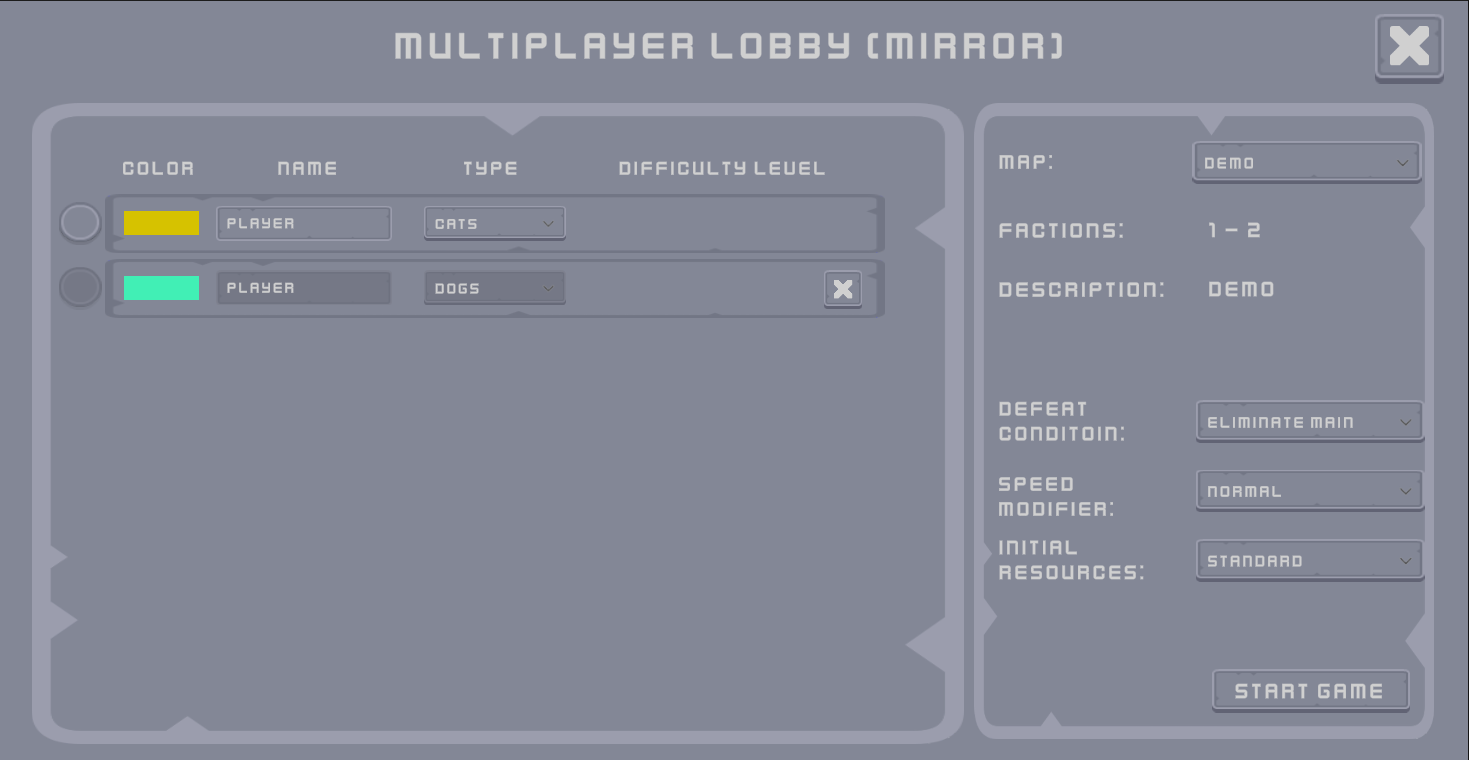
\includegraphics[width=\linewidth]{joingamePage.png}
  \caption{หน้าเลือกเผ่าก่อนเริ่มเกม}
\end{figure}

\begin{figure}[h]
  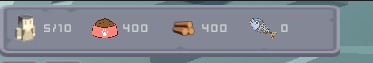
\includegraphics[width=\linewidth]{resource.png}
  \caption{Resource Bar}
\end{figure}

\enskip แต่ละเผ่าจะมีทรัพยากรพิเศษที่สามารถนําไปใช้ในการสร้าง Hero (unit พิเศษ) ได้ สําหรับเผ่า Doggy คือ กระดูก (Bone) ส่วนของเผ่า Kitty คือ ก้างปลา (Fishbone) ซึ่งทรัพยากรพิเศษทั้งสองนี้จะสุ่มวางตาม
พื้นที่ต่างๆ

\enskip ในการเล่นผู้เล่นจะต้องสร้าง unit พื้นฐานเพื่อใช้ในการเก็บรวบรวมทรัพยากร (Food, Wood, Bone/Fishbone)
นํามาสร้างสิ่งก่อสร้างต่างๆซึ่งใช้ในการสร้าง unit ต่อสู้แต่ละแบบและอัญเชิญ Hero ของฝั่งตัวเอง 
เพื่อที่ผู้เล่นจะได้ตั้งกองกําลังและนําไปบุกหรือตั้งรับฝั่งตรงข้าม

\enskip การสร้าง unit ของแต่ละฝั่งนั้นมีการสร้างได้จํานวนจํากัดผู้เล่นต้องทําการสร้างสิ่งก่อสร้าง 
นั่นก็คือ บ้าน เพื่อที่จะขยาย capacity ซึ่งมี limit ของการขยายอยู่ด้วย

\enskip เงื่อนไขในการชนะหรือแพ้ คือการที่ผู้เล่นฝั่งใดฝั่งหนึ่งสามารถทําลายฐานหลักของอีกฝั่งได้

\begin{figure}[ht]
  \centerline{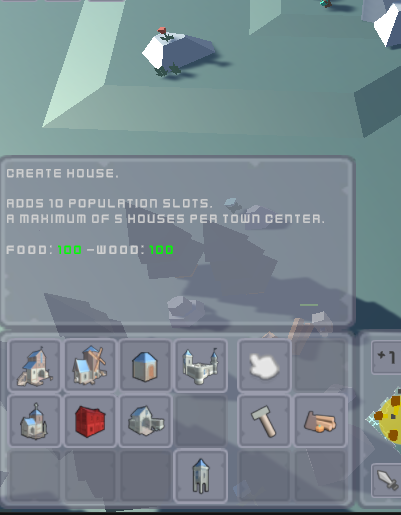
\includegraphics[scale=.7]{createBuilding.png}}
  \caption{แสดงเมนูการสร้าง building ของ unit พื้นฐาน}
\end{figure}

\begin{figure}[h]
  \centerline{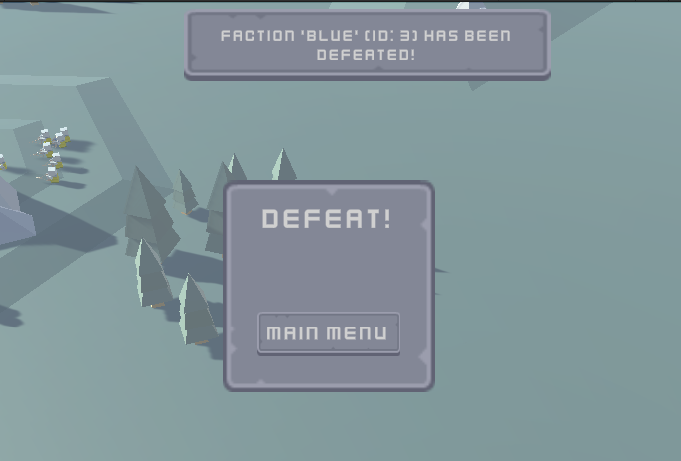
\includegraphics[scale=.6]{result.png}}
  \caption{แสดผลชนะ/แพ้ เมื่อทำลาย/ถูกทำลายฐานหลัก}
\end{figure}
\subsection{ระบบภายในเกม}

\begin{itemize}
  \item ระบบการสร้าง unit
  
  \qquad ในฐานหลักนั้นจะมีระบบการสร้างตัว unit พื้นฐานที่สามารถนําไปเก็บรวบรวมทรัพยากรได้ 
  และมีสิ่งก่อสร้างอื่นที่สามารถสร้าง unit ประเภทอื่นได้ เช่น Barrack สำหรับการสร้าง unit ต่อสู้
  \item ระบบสร้างสิ่งก่อสร้าง (building)
  
  \qquad ในการสร้างสิ่งก่อสร้าง จะให้ผู้เล่นใช้ตัว unit พื้นฐานในการสร้างสิ่งก่อสร้าง ซึ่งสิ่งก่อสร้างบางชนิดจะมีเงื่อนไขที่ต้องสร้างสิ่งก่อสร้างบางประเภทก่อนถึงจะทําการสร้างสิ่งก่อสร้างนั้นได้
  \item ระบบการต่อสู้
  
  \qquad ผู้เล่นสามารถทําการควบคุม unit ต่อสู้ / Hero เพื่อนําไปต่อสู้กับฝั่งตรงข้าม
  \item ระบบ Fog of War
  
  \qquad ใน map จะมีระบบซ่อนข้อมูลบนแผนที่ (Fog of War) ซึ่งทําให้ผู้เล่นต้องทําการสํารวจเพื่อเปิดเผยพื้นที่
  \item ระบบอัพเกรด unit
  
  \qquad ในเกมจะมีสิ่งก่อสร้างที่สามารถอัพเกรดตัว unit ต่อสู้ได้
  \item ระบบการขยาย capacity
  
  \qquad ผู้เล่นต้องทําการสร้างก่อสร้าง “บ้าน” เพื่อเพิ่มความจุในการสร้าง unit โดยรวมได้
\end{itemize}
\chapter{\ifproject%
\ifenglish Experimentation and Results\else การทดลองและผลลัพธ์\fi
\else%
\ifenglish System Evaluation\else การประเมินระบบ\fi
\fi}

\qquad ในบทนี้จะเป็นการทดสอบเกี่ยวกับระบบหลักๆในเกม และการประเมินผลลัพธ์

\section{วัตถุประสงค์ของการทดสอบ}
\begin{enumerate}
    \item ระบบหลักๆในเกม เช่นระบบการสร้าง unit, ระบบการสร้างสิ่งก่อสร้าง, ระบบการต่อสู้ สามารถทํางานได้อย่างถูกต้อง
    \item ผู้เล่นได้รับความบันเทิง ความสนุกสนาน จากการเล่นเกม Doggy Kitty War
\end{enumerate}

\section{การทดสอบโดยผู้เล่น}
\subsection{กลุ่มผู้เล่นเป้าหมาย}
\begin{itemize}
    \item กลุ่มนักเรียน-นักศึกษา
    \item ผู้ที่มีอายุระหว่าง 15-25 ปี
    \item ผู้ที่มีความสนใจในเกมกลยุทธ์ และชอบสุนัข/แมว
\end{itemize}
\subsection{ผลการทดสอบ}
จำนวนผู้ที่เข้าร่วมการทดสอบ \dots คน
\\การวัดระดับความพึงพอใจแบ่งเป็น 5 ระดับ
\\ระดับ 1 = น้อยที่สุด \quad ระดับ 2 = น้อย \quad ระดับ 3 = ปานกลาง \quad ระดับ 4 = มาก \quad ระดับ 5 มากที่สุด
\\
\begin{table}[ht]
\begin{center}
    \begin{tabular}{|p{3cm}m{3cm}m{3cm}m{3cm}m{3cm}m{3cm}p{3cm}p{3cm}p{3cm}p{3cm}p{3cm}p{3cm}p{3cm}p{3cm}p{3cm}p{3cm}p{3cm}p{3cm}|}
        \hline
        \multicolumn{1}{|c|}{\multirow{2}{*}{ลำดับที่}} & \multicolumn{1}{c|}{\multirow{2}{*}{รายการประเมิน}} & \multicolumn{15}{c|}{คะแนน} & \multicolumn{1}{c|}{\multirow{2}{*}{เฉลี่ย}} \\ \cline{3-17}
        \multicolumn{1}{|c|}{} & \multicolumn{1}{l|}{} & \multicolumn{3}{l|}{1} & \multicolumn{3}{l|}{2} & \multicolumn{3}{l|}{3} & \multicolumn{3}{l|}{4} & \multicolumn{3}{l|}{5} & \multicolumn{1}{l|}{} \\ \hline
        \multicolumn{1}{|c|}{1} & \multicolumn{1}{l|}{เกมโดยรวมมีความสนุกสนาน} & \multicolumn{3}{l|}{} & \multicolumn{3}{l|}{} & \multicolumn{3}{l|}{} & \multicolumn{3}{l|}{} & \multicolumn{3}{l|}{} & \multicolumn{1}{l|}{} \\ \hline
        \multicolumn{1}{|c|}{2} & \multicolumn{1}{l|}{การควบคุมง่ายและลื่นไหล} & \multicolumn{3}{l|}{} & \multicolumn{3}{l|}{} & \multicolumn{3}{l|}{} & \multicolumn{3}{l|}{} & \multicolumn{3}{l|}{} & \multicolumn{1}{l|}{} \\ \hline
        \multicolumn{1}{|c|}{3} & \multicolumn{1}{l|}{เสียงภายในเกมเหมาะสมกับเกม} & \multicolumn{3}{l|}{} & \multicolumn{3}{l|}{} & \multicolumn{3}{l|}{} & \multicolumn{3}{l|}{} & \multicolumn{3}{l|}{} & \multicolumn{1}{l|}{} \\ \hline
        \multicolumn{1}{|c|}{4} & \multicolumn{1}{l|}{กราฟฟิกของเกมมีความสวยงาม} & \multicolumn{3}{l|}{} & \multicolumn{3}{l|}{} & \multicolumn{3}{l|}{} & \multicolumn{3}{l|}{} & \multicolumn{3}{l|}{} & \multicolumn{1}{l|}{} \\ \hline
        \multicolumn{1}{|c|}{5} & \multicolumn{1}{l|}{ระบบโดยรวมของเกมทำงานถูกต้อง} & \multicolumn{3}{l|}{} & \multicolumn{3}{l|}{} & \multicolumn{3}{l|}{} & \multicolumn{3}{l|}{} & \multicolumn{3}{l|}{} & \multicolumn{1}{l|}{} \\ \hline
        \multicolumn{17}{|c|}{รวมคะแนนเฉลี่ย} & \multicolumn{1}{c|}{} \\ \hline
    \end{tabular}
    \caption{ตารางแสดงผลคะแนนเฉลี่ยความพึงพอใจ}
\end{center}
\end{table}
\subsection{สรุปผลความพึงพอใจ}
\ifproject
% \chapter{\ifenglish Conclusions and Discussions\else บทสรุปและข้อเสนอแนะ\fi}

\section{\ifenglish Conclusions\else สรุปผล\fi}



\section{\ifenglish Challenges\else ปัญหาที่พบและแนวทางการแก้ไข\fi}

ในการทำโครงงานนี้ พบว่าเกิดปัญหาหลักๆ ดังนี้

\section{\ifenglish%
Suggestions and further improvements
\else%
ข้อเสนอแนะและแนวทางการพัฒนาต่อ
\fi}

\fi

\nocite{*}
\bibliography{sampleReport}

\ifproject
\normalspacing
% \appendix
% \include{chapters/appendix}

%% Display glossary (optional) -- need glossary option.
\ifglossary\glossarypage\fi

%% Display index (optional) -- need idx option.
\ifindex\indexpage\fi

% \begin{biosketch}
% \begin{center}
%   \includegraphics[width=1.5in]{mugshot.jpg}
% \end{center}
% Your biosketch goes here. Make sure it sits inside
% the \texttt{biosketch} environment.
% \end{biosketch}
\fi % \ifproject
\end{document}
